\section{F77/F90xml implementation}
% {{{
The F77/F90xml library \cite{f77f90xml-site} is a C library designed to
provide a Fortran interface to libgdome2 \cite{gdome2-site}, an opensource
library (also developed using C language) part of the GNOME
\cite{gnome-site} project. Most of the design is implemented to give access
to a DOM level 2 interface \cite{w3-dom-level-2-site}, with the exclusion of
events, which are not needed in the target environment. XPath support is
available, although no testing has been performed and therefore must be
considered experimental.

At the time of writing, F77/F90xml library depends on libgdome2-0.8.0,
glib-1.2.10 \cite{glib-site}, libxml2-2.5.11 \cite{libxml2-site}.  Building
of the library also depends on Python 2.3 \cite{python-site} or above.  The
library has been successfully compiled on Intel/AMD Linux platform, with gcc
and Intel Fortran Compiler, and IBM SP4 with the xlf compiler suite. It is
released under the terms of the LGPL \cite{lgpl-site}.

F77/F90xml has been designed with Fortran 77 backward compatibility in mind.
The library provides two interfaces: a Fortran 90/95 interface, similar to
DOM Level 2 in order to reduce the need for specialized documentation, and a
Fortran 77 interface, using specialized subroutines named
\textit{multiplexers}.

The Fortran 77 interface is particularly complex and error prone.  An
experimental preprocessor has been deployed to translate pseudo-F90 code
into F77 code, but Fortran 77 is very old and the choice for new code should
be Fortran 95. Support for this language was an initial request from the
interested parties, and provides full freedom even to those projects that
still work in a pure Fortran 77 environment for their maintenance. 

When the library development started, no stable and free Fortran 90/95
compiler existed, and most of the potentially interested parties had the
requisite to compile the code using the GNU F77 compiler.  This situation
changed with the release of g95 and gfortran, however the Fortran 77
interface is directly obtained from the implementation, simplifying rather
than making more difficult the development of the library.

In the following, we will refer to the Fortran 90 interface with the term
``F90xml'', and with ``F77xml'' to the specific Fortran 77 interface.
Finally, the term ``F77/F90xml'' refers to the library as a whole.
% }}}

\subsection*{The Fortran 90/95 interface}

The Fortran 90/95 interface provides a clean and simple access. All gdome2
functions are mapped to Fortran subroutines, collected together into a 
\texttt{MODULE}. A simple code example is provided 

{
\footnotesize
\begin{verbatim}
INTEGER :: first, last, elem, err

Comment <... get elem by some other call ...>

CALL f90xml_el_firstChild(first,elem,err)
CALL f90xml_el_lastChild(last,elem,err)
\end{verbatim}
}

which can be compared with the equivalent C code

{
\footnotesize
\begin{verbatim}
GdomeElement *elem;
GdomeNode *first, *last;
GdomeException exc;

/* <... get elem by some other call ...> */

first = gdome_el_firstChild(elem, exc);
last = gdome_el_lastChild(elem, exc);
\end{verbatim}
}

This comparison presents the main featured differences of the F90xml usage
with respect to gdome2. Apart of the routine names, where the standard
prefix ``\texttt{gdome\_}'' is replaced with ``\texttt{f90xml\_}'', two
major differences exist. 

The first difference is bound to the data reference handling.  The C
interface provided by gdome2 is structured in {Object Oriented} style.
Routines handle pointers to structures, dynamically allocated inside the
library. 

To prevent issues relative to the handling of memory pointers
between C and Fortran, the F77/F90xml library provides a simple mapping
between an integer value and a memory pointer (for example to
\texttt{GdomeNode}, \texttt{GdomeDOMString},
\texttt{GdomeDomImplementation}, and so on).  Fortran client code always
handle these integers, hereafter named
\textit{codes}, univocally identifying a particular gdome pointer.  The
F77/F90xml library internally implements a cache to store these pointers and
the corresponding code, providing an internal facility to obtain codes from
memory pointers and viceversa.  The current implementation of the library
uses a simple linked lists to store the mapping, and this correspondence is
kept until the gdome2 object is completely deallocated.  Substitution of the
linked list with a more efficient hash table can be implemented
transparently.

The second major difference is the arguments layout: in F90xml, the
first argument of the subroutine is the gdome2 returned value, therefore the
{Fortran~90} interface declares this argument as \texttt{INTENT(OUT)}. The
subsequent arguments are the requested gdome2 arguments, marked as
\texttt{INTENT(IN)} in the {Fortran~90} interface, with the
exception of the last one, holding the returning error condition and
therefore marked as \texttt{INTENT(OUT)}. 

If the gdome2 function returns \texttt{void} (no value), the corresponding
F90xml subroutine accepts an integer as a first argument. On return, this
value is set to the standard numeric parameter \texttt{NullCode}, which
evaluates to zero. 

\subsection*{String handling}

For most of the time, strings in F77/F90xml are handled as codes
representing \texttt{DOMString} objects: when an element name is requested,
the F77/F90xml subroutine returns a code referencing a \texttt{DOMString}
object. Setting an element name or TextNode data requires passing a
\texttt{DOMString} code. A set of routines has been provided to simplify the
handling of these objects:
\begin{itemize}
\item \texttt{f90xml\_str\_mkref}: creates a new \texttt{DOMString} from a Fortran
\texttt{CHARACTER} string. Accepts the Fortran string and returns a code referencing
the newly created \texttt{DOMString} object.
\item \texttt{f90xml\_str\_length}: accepts the code of the \texttt{DOMString} and
returns the length of the string.  This routine can be useful to know in
advance how many bytes are needed to read from the \texttt{DOMString}, and act
accordingly. A classical example could be a \texttt{DOMString} containing 300 bytes
and the Fortran code has a \texttt{CHARACTER(LEN=100)} available.
\item \texttt{f90xml\_str\_toFortran}: extracts Fortran character
data from an existing \texttt{DOMString} object. This routine accepts the code of the
\texttt{DOMString}, a \texttt{CHARACTER(LEN=*)} variable, an \texttt{INTEGER} offset
and returns a \texttt{LOGICAL} value. The \texttt{DOMString} data will be extracted
starting at the position provided by the zero-based offset. No more than
the length of the \texttt{CHARACTER} variable will be extracted from the
\texttt{DOMString}. The returned \texttt{LOGICAL} value is set to \texttt{.TRUE.} if the
\texttt{DOMString} has been extracted up to the last character, otherwise
\texttt{.FALSE.}. Using the returned logical value and working with
appropriate offsets, it is possible to read long strings in a chunked
fashion, regardless of the effective dimensions of the \texttt{DOMString} and
\texttt{CHARACTER} variable.
\item \texttt{f90xml\_str\_print}: Prints the \texttt{DOMString} to standard
output. Returns \texttt{void}. 
\item \texttt{f90xml\_str\_equal}: Performs a comparison between
a \texttt{DOMString} referenced by its code and a Fortran \texttt{CHARACTER} string.
Returns \texttt{.TRUE.} if the strings are equal, otherwise \texttt{.FALSE.}
\item \texttt{f90xml\_str\_unref}: deletes the \texttt{DOMString}. Returns
\texttt{void}.
\end{itemize}

\subsection*{Errors}

The F77/F90xml library returns the error status \textit{via} the last
\texttt{INTEGER} argument. The returned value depends on the kind of error,
and a list of \texttt{PARAMETER}s account for all the available situations.
The \texttt{ERR\_NO\_ERROR} value, which evaluates zero, is returned if no
error occurs. The library checks for various error conditions, such as
\begin{itemize}
\item a passed code is not of the expected type, after inquiry into the cache
(e.g. passing the code corresponding to \texttt{DOMString} to
\texttt{f90xml\_el\_firstChild})
\item a code does not reference to any cached object
\item a \texttt{NullCode} is passed to a routine unable to handle it
\item internal errors of the gdome2 library
\end{itemize}

\subsection*{Library architecture and Fortran 77 interface}

Standard Fortran 77 expects names limited to 6 characters, although at our
knowledge no recent Fortran 77 compiler imposes this strict limit. Deploying
the complete DOM interface with a one-to-one mapping in such limited
namespace would result in name collisions and routine names with no meaning.

To face this issue, a few multipurpose C functions have been created, named
\textit{multiplexers}.  The role of each multiplexer is to create a
many-to-one correspondence between a subset of the gdome2 routines accepting
the same number and type of arguments and the single generic multiplexer
function. Multiplexers give access to the complete interface with a reduced
namespace footprint.

Each C multiplexer is directly mapped by the library to a F77
\texttt{SUBROUTINE}, in a one-to-one relationship.  Code between the Fortran
frontend and the corresponding C multiplexer is needed to interface these
two languages and their different standards for string handling, memory
management, routine name mangling and parameters. 

The multiplexers are the core of the library. When a multiplexer is
called, it dispatches (demultiplexes) the call to the appropriate function
of the subset it describes. In turn, this function performs the actual call
to the gdome2 routine. To select which routine to call, a string containing
the name of the routine is passed as an argument. Internally, this information
is used to invoke the correct function.  Fig. \ref{fig:f77xml-high-level}
represents a high-level view of a single multiplexer. 

Each multiplexer routine and its Fortran interface have a standardized name,
bound to the number and type of arguments it accepts.

A schematic classification of the routines has been devised to describe with
a short notation the number and type of accepted parameters, and the
returned value.  Routines with the same type signature are handled by the
same multiplexer.  The core implementation resorts on the equality of
signatures to collect pointers to functions. 

In the following, a textual representation of the signature will be written
in the compact form \texttt{(return|arguments)}.  For each kind of argument,
a letter has been assigned: ``\texttt{c}'' for code, ``\texttt{b}'' for
boolean (logical), ``\texttt{e}'' for error, ``\texttt{s}'' for string,
``\texttt{u}'' for unsigned integer.  Also, the ``\texttt{v}'' is used with
subroutines that return no value (are \texttt{void} in C syntax). 

As an example, all the gdome2 functions given below

{
\footnotesize
\begin{verbatim}
GdomeNode* gdome_el_firstChild(GdomeElement *self, GdomeException *exc);

GdomeElement* gdome_doc_documentElement(GdomeDocument *self, GdomeException *exc);

GdomeNode* gdome_el_lastChild(GdomeElement *self, GdomeException *exc);
\end{verbatim}
}
accept a code and an error and return a code. The signature of these
functions therefore is \texttt{(c|ce)} and they are handled by the
same multiplexer.  The associated Fortran entry point is the subroutine
\texttt{xp3t1}, where ``\texttt{x}'' is a standard prefix, ``\texttt{p3}''
(literally ``parameters 3'') denotes the number of arguments involved in the
signature (two codes and the error) and ``\texttt{t1}'' (literally, ``type
1'') is bound to the type of the arguments.  The type is needed to
distinguish routines that accept 3 parameters of a different type.  For
example, the following routine 
\begin{center}
\begin{figure}[t]
\begin{center}
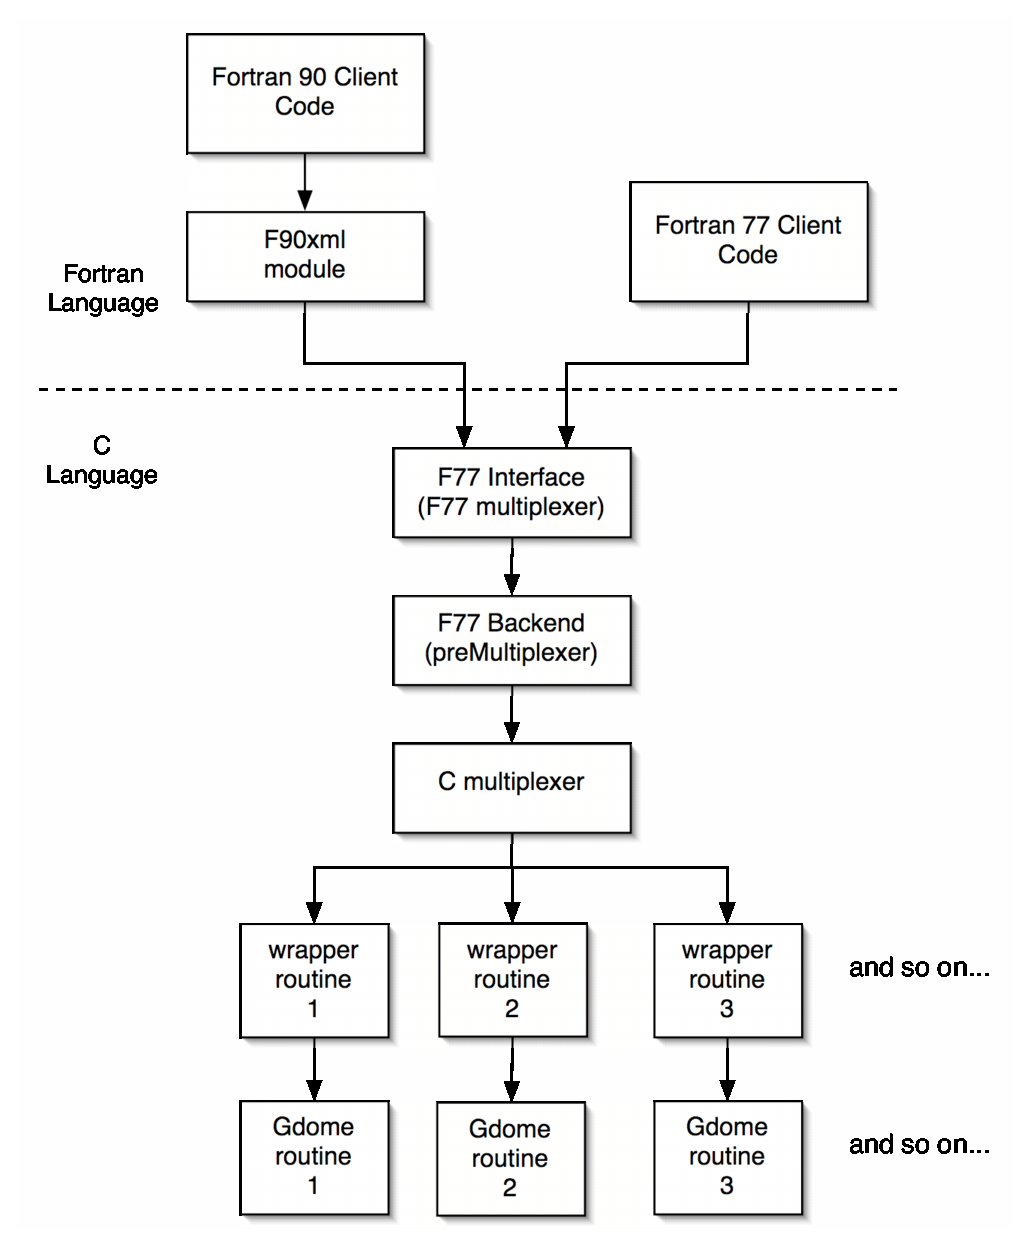
\includegraphics[width=100mm,keepaspectratio]{04_grid/images/f77xml-high-level-gimped.eps}
\end{center}
\caption{\footnotesize A graphical scheme representing the F77/F90xml
library structure. Each multiplexer groups a high number of gdome2
subroutines.}
\label{fig:f77xml-high-level}
\end{figure}
\end{center}

{
\footnotesize
\begin{verbatim}
GdomeBoolean gdome_el_hasChildNodes(GdomeElement *self, GdomeException *exc);
\end{verbatim}
}
has signature \texttt{(b|ce)} and is handled by a multiplexer with the same
\texttt{p} value but different \texttt{t} value: \texttt{xp3t4}

An exception is represented by routines returning \texttt{void},
\texttt{(v|ce)}. These routines are handled as \texttt{(c|ce)} routines,
accepting a dummy return argument which is set to the special value
\texttt{NullCode}. In other terms, both \texttt{(c|ce)} and \texttt{(v|ce)}
routines are managed by the same multiplexer, the \texttt{xp3t1} multiplexer.
It must be pointed out that no matching scheme exists to obtain the type
number from the letter sequence in the signature. 

The \texttt{xp3t1} multiplexer by itself maps and gives access to
approximatively 240 gdome2 functions. The complete DOM interface (more than
450 functions) is mapped by 21 multiplexers. As already said, the
gdome routine is chosen by the means of a \texttt{CHARACTER} argument which
is passed to the multiplexer.  By convention, this argument is passed
between the return value and the first \texttt{INTENT(IN)} argument,
therefore always in the second position. 

As a final result, the Fortran 77 interface to the multiplexer is
represented in the example below

{
\footnotesize
\begin{verbatim}
       CHARACTER*128 fnName
       INTEGER first, last , elem, err

Comment <... get elem by some other call ...>

       fnName='el_firstChild'
       CALL xp3t1(first,fnName,elem,err)

       fnName='el_lastChild'
       CALL xp3t1(last,fnName,elem,err)
\end{verbatim}
}
As can be seen from the example, the function name is case sensitive and is
the exact copy of the gdome2 function, stripped of the ``\texttt{gdome\_}''
prefix.  The Fortran 90 module provides long named subroutines performing
the mapping between each subroutine and the corresponding multiplexer.

The library architecture here presented was chosen for two reasons: 
\begin{itemize}
\item reduce the development cost, providing automatized creation of the
library
\item keep potential Fortran 77 compatibility.
\end{itemize}

A large part of the library is developed in XML. An XML file contains all
the informations to create the binding routines called from the C
multiplexers.  The file is parsed by a Python script which
collects the needed informations, and deploys the C and Fortran code. 

The logic involved is to define templates for the binding routines, and to
replace ad-hoc placeholder keywords with appropriate entries for the
specific routine. When a particular specific implementation cannot be
generated by a template, the format allows to override the template
mechanism and to pass the specific implementation.

We can note that the Fortran 77 interface is a direct subproduct of the
internal implementation of the library, therefore is convenient to deploy it
even if not used by client code. 

%In order to simplify the cleanup of the allocated structures, the
%\textt{f90xml_cache_flush} routine is provided. Using this routine the
%client code can delay the cleanup of many objects to a single final call.
%Functions for unreferencing single structures (Nodes, DOMStrings etc...) are
%also available at F77/F90xml level.
%
%{
%\footnotesize
%\begin{verbatim}
%CHARACTER(LEN=4) :: fortranString
%\end{verbatim}
%}
%
%and accessing the \texttt{f90xml\_str\_toFortran} routine with fortranString and
%offset 0, fortranString will contain "Here" and the returned logical value will
%be \texttt{.FALSE.}. With an offset of 5, fortranString will contain "is t", and
%again the returned logical value will be \texttt{.FALSE.}. Finally, with an offset
%of 13, fortranString will contain "ata" and the returned logical value will
%be \texttt{.TRUE.}. 
%{
%\footnotesize
%\begin{verbatim}
%0 : ERR_NO_ERROR 
%\end{verbatim}
%}
%
%
%{
%\footnotesize
%\begin{verbatim}
%10 : ERR_DATA_NOT_AN_ELEMENT 
%11 : ERR_DATA_NOT_A_NODE  
%12 : ERR_DATA_NOT_A_DOCUMENT 
%13 : ERR_DATA_NOT_A_STRING  
%14 : ERR_DATA_NOT_A_NODELIST 
%15 : ERR_DATA_NOT_A_COMMENT  
%16 : ERR_DATA_NOT_AN_ATTR 
%17 : ERR_DATA_NOT_A_NAMEDNODEMAP 
%18 : ERR_DATA_NOT_A_TEXT     
%19 : ERR_DATA_NOT_AN_ENTITYREF  
%20 : ERR_DATA_NOT_AN_ENTITY 
%21 : ERR_DATA_NOT_A_PROCESSINGINSTRUCTION  
%22 : ERR_DATA_NOT_A_CDATASECTION 
%23 : ERR_DATA_NOT_A_DOCUMENTFRAGMENT
%24 : ERR_DATA_NOT_A_DOCUMENTTYPE   
%25 : ERR_DATA_NOT_A_DOMIMPLEMENTATION  
%\end{verbatim}
%}
%
%These errors are returned every time a passed code is not of the expected type, after inquiry into the cache.
%For example passing the code that corresponds to a DOMImplementation to
%f90xml\_el\_firstChild, a ERR\_DATA\_NOT\_AN\_ELEMENT is returned, because f90xml\_el\_firstChild expects an element.
%It is important to note that a code referring to an Element can be passed to Node handling
%subroutines like f90xml\_n\_appendChild (which accept a code for a node),
%because in the DOM abstraction an Element is a specialization of a Node.
%
%{
%%\footnotesize
%\begin{verbatim}
%30 : ERR_NO_CACHE_HIT
%\end{verbatim}
%}
%
%This error is returned when a given code does not reference to any object in
%the cache. This usually is indicative of a bug in the client code.
%
%{
%\footnotesize
%\begin{verbatim}
%31 : ERR_NULL_CODE
%\end{verbatim}
%}
%
%This error is returned when a NullCode is passed to a routine unable to
%handle it.
%
%{
%\footnotesize
%\begin{verbatim}
%1000 : ERR_NEVER_RETURN_THIS
%\end{verbatim}
%}
%
%A watchdog error value. No routine should return this error. If this
%happens, a library bug is the cause.
%
%{
%\footnotesize
%\begin{verbatim}
%10000: ERR_GDOME
%\end{verbatim}
%}
%
%An error at gdome2 level has been detected. A F77/F90xml library bug can
%trigger this error.
